%%%%%%%%%%%%%%%%%%%%%%%%%%%%%%%%%%%%%%%%%%%%%%%%%%%%%%%%%%%%%%%%%%%%%%%%%%%%%%%%
%2345678901234567890123456789012345678901234567890123456789012345678901234567890
%        1         2         3         4         5         6         7         8

\documentclass[letterpaper, 10 pt, conference]{ieeeconf}  % Comment this line out if you need a4paper
\usepackage{amsmath, xparse}
\usepackage{amstext}
\usepackage{amsfonts}
\usepackage{float}
\usepackage{graphicx}
\usepackage{hyperref}
\usepackage[utf8]{inputenc}
\usepackage{algorithm}
\usepackage[noend]{algpseudocode}
\usepackage{caption}
\usepackage{adjustbox}
\usepackage{booktabs}
\usepackage{outlines}

\makeatletter
\renewcommand{\Function}[2]{%
  \csname ALG@cmd@\ALG@L @Function\endcsname{#1}{#2}%
  \def\jayden@currentfunction{#1}%
}
\newcommand{\funclabel}[1]{%
  \@bsphack
  \protected@write\@auxout{}{%
    \string\newlabel{#1}{{\jayden@currentfunction}{\thepage}}%
  }%
  \@esphack
}
\makeatother

%\documentclass[a4paper, 10pt, conference]{ieeeconf}      % Use this line for a4 paper

\IEEEoverridecommandlockouts                              % This command is only needed if
                                                          % you want to use the \thanks command

\overrideIEEEmargins                                      % Needed to meet printer requirements.

%In case you encounter the following error:
%Error 1010 The PDF file may be corrupt (unable to open PDF file) OR
%Error 1000 An error occurred while parsing a contents stream. Unable to analyze the PDF file.
%This is a known problem with pdfLaTeX conversion filter. The file cannot be opened with acrobat reader
%Please use one of the alternatives below to circumvent this error by uncommenting one or the other
%\pdfobjcompresslevel=0
%\pdfminorversion=4

% See the \addtolength command later in the file to balance the column lengths
% on the last page of the document

% The following packages can be found on http:\\www.ctan.org
%\usepackage{graphics} % for pdf, bitmapped graphics files
%\usepackage{epsfig} % for postscript graphics files
%\usepackage{mathptmx} % assumes new font selection scheme installed
%\usepackage{times} % assumes new font selection scheme installed
%\usepackage{amsmath} % assumes amsmath package installed
%\usepackage{amssymb}  % assumes amsmath package installed

\title{\LARGE \bf
AlienGLRenderer: A simple 3D OpenGL renderer for simple scenes
}



\author{Arrian Chi% <-this % stops a space
\\
\\ % TODO TODO
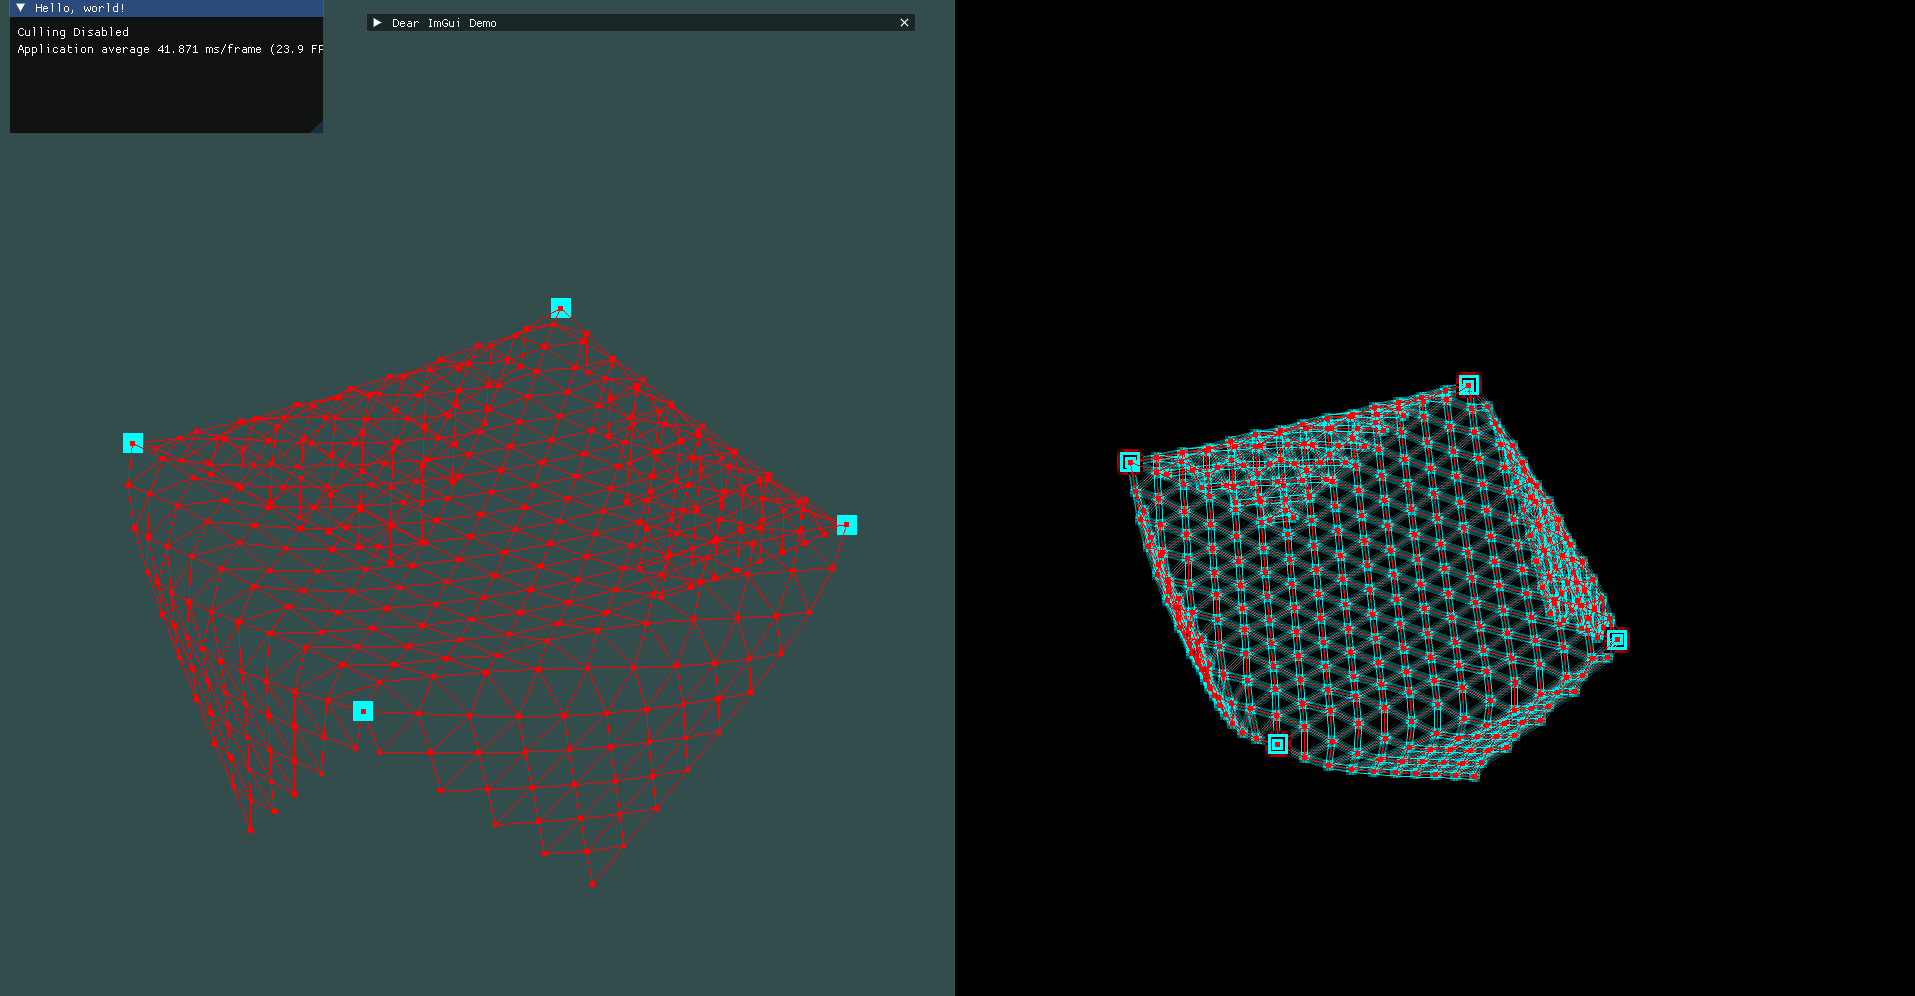
\includegraphics[width=8.7cm]{cloth1.PNG} \> 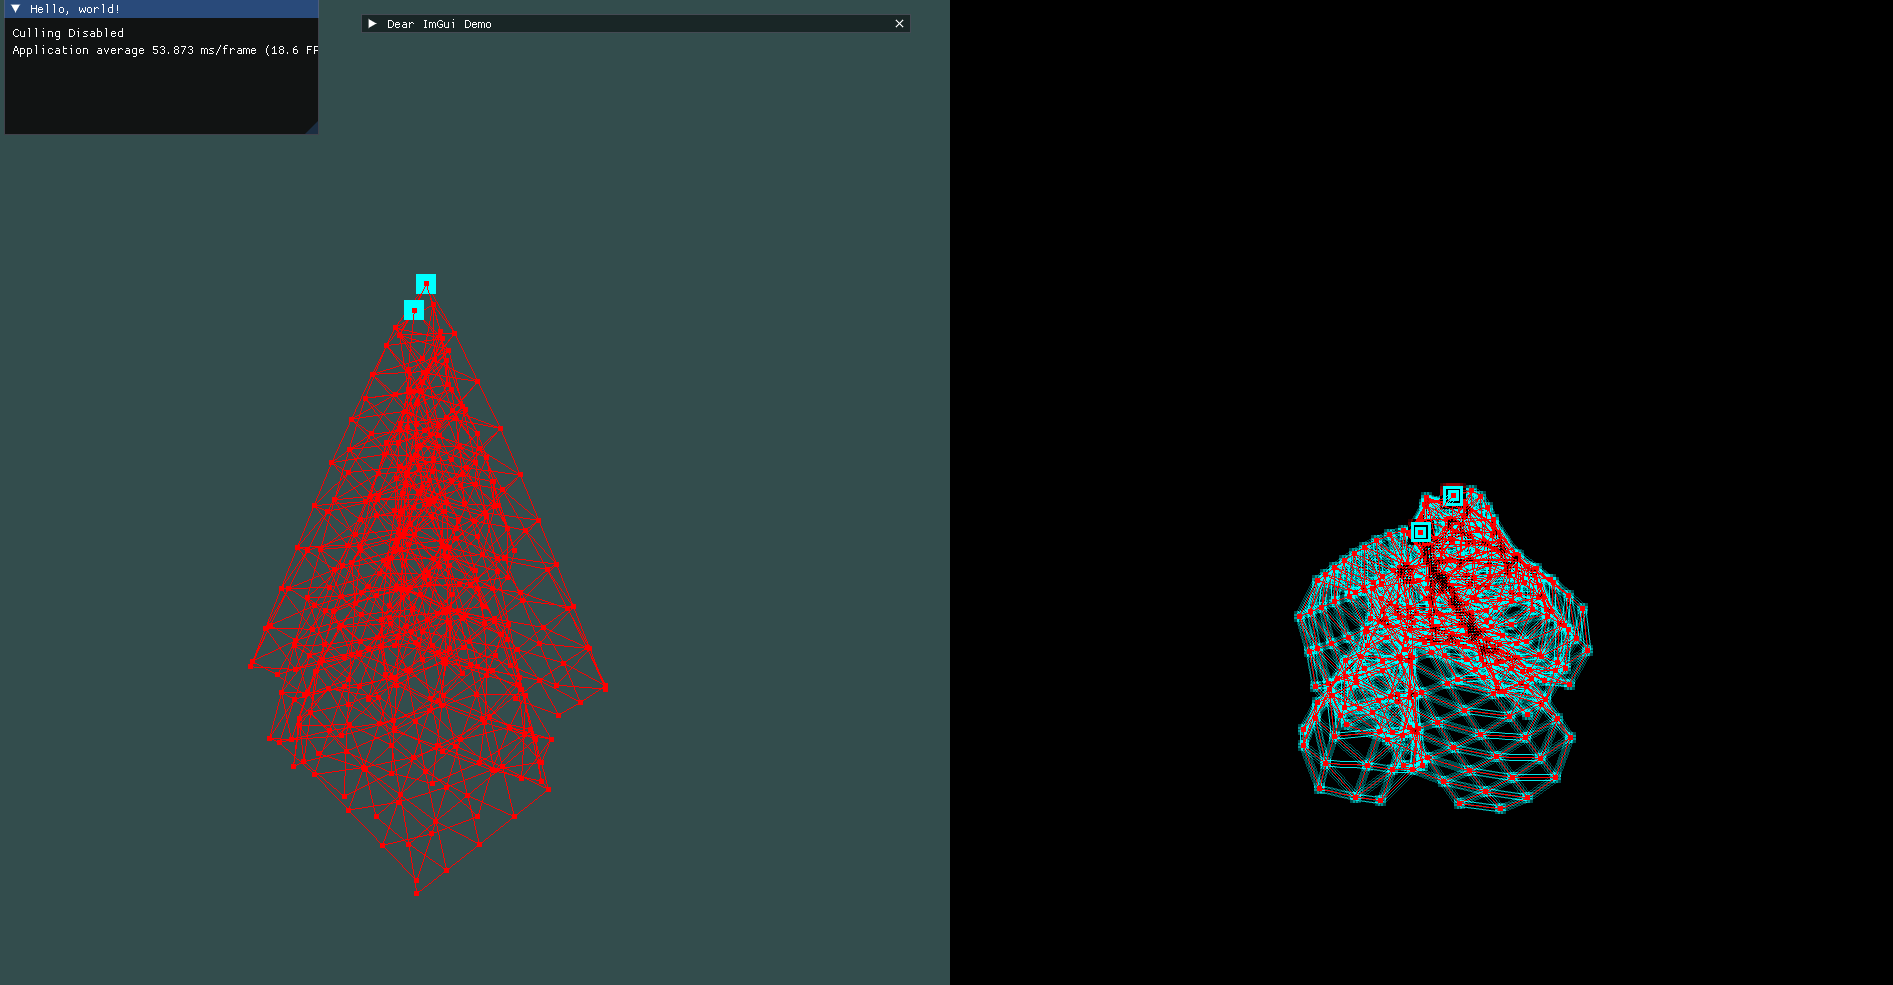
\includegraphics[width=8.7cm]{cloth2.PNG} 
}




\begin{document}

% \onecolumn


\maketitle
\thispagestyle{empty}
\pagestyle{empty}


%%%%%%%%%%%%%%%%%%%%%%%%%%%%%%%%%%%%%%%%%%%%%%%%%%%%%%%%%%%%%%%%%%%%%%%%%%%%%%%%

\begin{abstract}

AlienGLRenderer is a renderer, written in C++ and OpenGL, designed to support the creation of simple scenes (inspired by the Quake Engine). The overall goal of this project is to streamline the rapid creation of simple scenes for artistic expression and to showcase evidence of technical knowledge. In this report, I showcase what features have been implemented, the technical challenges faced, and the future work to improve the renderer. 

\end{abstract}
\section{Overview}
Computer graphics is a field of computer science involved in the manipulation of data to generate visual content on a computer. Some may call it esoteric in the way that it combines a variety of paradigms from other fields of study, such as math, optics, and physics, for the overarching goal of producing purposeful images on a screen. Its applications in the film industry, the video game industry, and even in scientific visualization prove its importance in our society. 

AlienGLRenderer is a hobby project implemented in OpenGL and C++ that I started in the summer of 2024 in hopes of pursuing a career in computer graphics. The project was inspired by the Quake Engine, a game engine developed by id Software in the 1990s. The engine was known for its simplicity and ease of use, which made it a popular choice for modders and indie developers. I wanted to create a similar engine that would allow me to experiment with graphics features and improve my skills in C++ and OpenGL, and also enable me to create simple graphics scenes in a easily configurable format.

In this paper, I would like to demonstrate the knowledge I have attained from the genesis of the project till now. I will discuss the process of the implementation of the renderer, the technical challenges I have faced through the course of its creation, and what future lies ahead for this renderer (including any remarks I have about OpenGL in the modern age).

\subsection{Design}
In the past, I have used OpenGL in a few other projects. The issue I found with these projects was that they were 1) too unoptimized and 2) hard to maintain. A few common tropes I found in these projects was encapsulation of rendering logic to the objects to be rendered (that is I implemented a render function for every cube, every sphere, etc.) and the frequent rebinding of buffers, shaders, and assets to render different objects (a buffer was initialized for every rendering primitive...). These issues arose from the blind usage of code from tutorials and introductory classwork and the misconception that object-oriented programming was the best way to conceptualize code. 

The OpenGL API can be understood as a state machine that uses its current state to perform rendering tasks \cite{openglconcepts}. The user must bind state (buffers, shaders, textures, etc. all represented by an ID) to the OpenGL context before performing draw calls. One may conceptualize it like a switchboard, where the operator (the programmer) must switch the connections (the OpenGL state) to get the desired output (the rendered image). The reason the API is designed this way is a result of the history of graphics hardware (which could be expanded upon in its own paper). Simply put, graphics hardware started out with using fixed function pipelines that were highly customizable but required manual configuration \cite{Peddie_2022}. The OpenGL API served as a high-level abstraction implemented by hardware vendors to allow programmers to configure the hardware without needing to know the specifics of the hardware. 

So naturally, if one tries to religiously use object-oriented paradigms to encapsulate rendering logic, they would end up with a lot of overhead. For example, let us imagine we have a scene with many cubes, each having their own transforms. The naive programmer probably do this: for each object, bind its mesh data and transformation matrices to the OpenGL context. Then, issue a draw call to the GPU. 

Note all this data lives in CPU RAM and must be copied to the GPU for it to be used. But CPU to GPU memory latency is relatively high. So if you are sending data to the GPU individually for every object, you are waiting for the GPU to finish rendering the object before you can send the next object. The CPU would be stalling while waiting for the GPU to finish rendering, resulting in significant overhead and bottlenecks. 

Luckily, the OpenGL API permits the batching of state to minimize draw calls and memory transfers. In our example, the programmer would recognize that all cubes used the same mesh but had different transformations, so they instance all the cubes with the same mesh data and send every transformation matrix at once in a large matrix buffer to the GPU. In the vertex shader, the appropriate transformation matrix would be indexed and used for world space to model space transformations. This would reduce the number of draw calls and memory transfers, thus reducing the overhead.

The aggregation of state to reduce high latency computation is a common optimization technique in computer graphics and is used in many modern game engines. However, it requires that the architecture of the renderer be data-oriented (separating logic and data) rather than object-oriented (combining data and behavior). Thus, I decided that the renderer would be designed such that it knew about how to render every object primitive that could be renderered in a scene. This provides me with a lot of flexibility in how I can render objects and manipulate draw calls, which I will demonstrate when I discuss the features of the renderer. Note that I am not completely abandoning object-oriented programming, but rather thinking more about the data the application is manipulating. 


\section{Features Implemented}

\subsection {Renderer Mainloop}
As mentioned before, I did not completely abandon object-oriented programming in the development of this renderer. The \texttt{Renderer} object itself contains all the data and logic needed to render a \texttt{Scene} object. A \texttt{Scene} object is a collection of data structures containing all the objects in a \texttt{SceneData} object that the renderer may directly read and use when rendering. A \texttt{SceneData} object contains that holds the uncompressed data read from a \texttt{.scn} file. Finally, \texttt{.scn} files are raw map data files (with a similar format to the Quake map format \cite{quake}) that contain all the scene objects and their properties. The static class containing the logic to load a \texttt{SceneData} from a \texttt{.scn} file and a \texttt{Scene} from a \texttt{SceneData} is called the \texttt{SceneLoader}.

To explain the algorithm of the render loop, the user supplies a path to the \texttt{.scn} file they want to render, which gets converted into a \texttt{Scene} object. The \texttt{Renderer} object is created and initialized with the size of framebuffer textures the renderer will render onto (more on this when discussing post-processing). While the window is open (the user has not closed the window), the application will first update the scene (which includes updating the camera, updating the cloth simulation, etc.), then call \texttt{renderer.render(scene)} for every renderer initialized. The application will then take each renderer's framebuffer texture and render it onto the main framebuffer texture. After that, the application will render any UI elements (using ImGui) on top of the main framebuffer texture. Finally, the application will swap the buffers, poll for events, and repeat the process.

\subsection{What is done in the \texttt{renderer.render(scene)} call?}
The \texttt{renderer.render(scene)} call is the most important call in the mainloop. It is where the renderer will render the scene onto the framebuffer texture. The renderer will first update the camera (if the camera is not locked), then update the cloth simulation (if the cloth simulation is enabled). The renderer will then iterate through all the rendering tasks in the scene and render them.


\subsection {Direct State Access (DSA)}
I previously stated that the OpenGL API is a state machine that requires the programmer to modify it to perform rendering tasks. In the past, this was not only limited to drawing, but also the manipulation of data. The programmer would bind the buffer to the global context, do whatever modifications they needed to the buffer, and then unbind it when not in use \cite{StephanoDSA}. This is no different than being limited to a set number of global registers you are forced to use to modify your data. This could quickly become an issue because logic in different parts of the application must share the same global state in order to modify data in their local scope. This is a big problem especially if the app is organized in an object-oriented fashion.

Direct state access is a feature introduced in OpenGL 4.5 that allows the programmer to modify OpenGL objects without needing to bind them to the global context. . The relevant calls to this are \texttt{glCreateBuffers}, \texttt{glNamedBufferStorage}, and \texttt{glNamedBufferSubData}, which creates a buffer, allocate memory for the buffer, and modifies the data for the buffer, respectively. Semantically, these calls treat each buffer as its own piece of data, independent of the global state. All that is needed is the buffer's name, which is generated by \texttt{glCreateBuffers} to be used by other calls to identify the buffer of interest to use. In AlienGLRenderer, I use DSA for all data buffers (vertex, index, uniform, frame, etc.) to reduce the overhead of binding and unbinding buffers for every object to be rendered. 


\begin{figure}
        \centering
        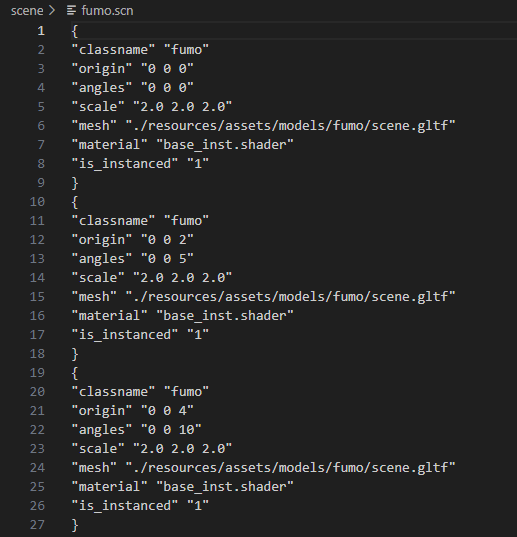
\includegraphics[width=0.45\textwidth]{scn.PNG}
        \caption{An example of the \texttt{.scn} file format} \label{fig:scn}
\end{figure}


\subsection {Scene Loading}
AlienGLRenderer's scene loading was inspired by that of the Quake Engine and its relatives \cite{quake}. Fig. \ref{fig:scn} shows an example file format of the \texttt{.scn} file. The format is pretty straightforward; every object in the scene stores its data as a series of key value pairs (kvps). The currently supported kvps include \texttt{classname}, \texttt{origin} (position), \texttt{angles}(rotation), \texttt{scale}, and \texttt{material}(currently just a shader name). The most important key is the \texttt{classname}, which is used to identify the object (i.e. a cube, an entity, a camera, etc.), which indicates how it should be processed.



\subsection{Instancing}
Briefly covered in the previous section, GPU instancing is the idea of drawing multiple copies of the same model mesh with slightly varying data all at once (i.e. blades of grass with varying heights/positions). In terms of draw calls, GPU instancing reduces several draw calls of the same mesh into one single draw call (\cite{Vries_2014}).  The benefit is that we reduce the expensive CPU to GPU communication overhead and the CPU stalls that come with it.

In the scene, entities (any object with a \texttt{classname} that does not have special handling) are the only objects that are instanced. It is your typical 3D object rendered into a scene consisting of a mesh, a shader, and a transform. The \texttt{SceneLoader} uses the concatenated mesh path and shader path as the key for an \texttt{entityInstanceMap} (really, should be called an \texttt{entityInstanceRenderTaskMap}). Each key is associated with an \texttt{EntityInstanceData} (should be called an \texttt{EntityInstanceRenderTask}), which aggregates all the entities with the same mesh and shader into a single rendering task. Each rendering task contains the instance count, a buffer of all the transformation matrices for each entity, the model data, and the shader data. The model data contains all the necessary meshes, materials, textures, and draw commands (more on this later) required to render its own mesh. So when the renderer is rendering the scene, it will iterate through all the rendering tasks and issue the draw calls with appropriate instancing data (i.e. the instance count and instance buffers). At first, this was done with \texttt{glDrawElementsInstanced}, but the call was later changed to \texttt{glMultiDrawElementsIndirect} to accomodate for indirect draws.

\subsection {Model Loading}
AlienGLRenderer currently only accepts \texttt{.glTF} files (graphics library transmission format) (\cite{GLTF}) as a valid model file. It leverages the fastgltf library to parse the \texttt{.glTF}. I decided to use the glTF file format because it stores data in the JSON format and use indices to reference data organized in the flat hierarchy ("scenes refer to root nodes by index, nodes refer to meshes (which are composed of primitives), which refer to materials, which refer to textures, which refer to images"). A static class named \texttt{ModelLoader} is responsible for loading the \texttt{.glTF} file and converting it into a \texttt{Model} object, creating the buffers for each category of data, as well as their indices. One key point to note is that every single \texttt{Model} is associated with a buffer of draw commands for each primitive (individual parts of a mesh) (more on this in the next section), the transforms of all nodes in the model, and a buffer of node primitive properties containing indices for the draw command to index the primitive's transform (that of the node their mesh is indiced in). (This really needs a figure). These draw commands are issued by \texttt{Renderer} per \texttt{EntityInstanceData} in the \texttt{Scene} when rendering, preserving the original transform hierarchy of the \texttt{.glTF} model.

\subsection {Indirect Draw Commands}
In pursuit of better performance (from both instancing and frustum culling), AlienGLRenderer uses indirect draw commands (\texttt{glMultiDrawElementsIndirect}) to render entities. When using indirect draw commands, draw calls are abstracted as command structs that contain parameters for the draw call (i.e. same parameters as \texttt{glDrawElements}). The command structs are stored in a buffer and sent to the GPU, and when \texttt{glMultiDrawElementsIndirect} is called, the GPU will submit draw calls for each struct in the buffer. This feature opens up the possibility of parallel draw command manipulation, either on the CPU (each thread can write to the command buffer) or the GPU (use the draw command buffer just like any buffer in a compute shader). In AlienGLRenderer, the latter case is showcased in the frustum culling feature to set the instance counts of every draw command in the buffer for an \texttt{entityInstanceData} struct. Every model has its own draw command buffer (a draw command for each primitive to be rendered) that stays on the GPU (no CPU readback) for the duration of the application's lifetime.

\subsection {Frustum Culling}
If rendering is the bottleneck of an application, it is common to reduce the amount of objects to be rendered using a culling algorithm, which filters draw calls based on the visibility of the primitives relative to the camera before they are issued to the GPU. There are 3 noteble culling algorithms: back-face culling (culling the polygons whose points are in the opposite winding order i.e. if counter-clockwise winding is front-facing, then all polygons with clockwise winding are culled), occlusion culling (culling primitives that are hidden, or occluded, behind other visible primitives closer to the camera), and frustum culling (culling primitives that are outside the view frustum of the camera). AlienGLRenderer implements frustum culling (see Fig. \ref{fig:cull}), and in the sections below, I will discuss my process of implementing it.

\begin{figure}
        \centering
        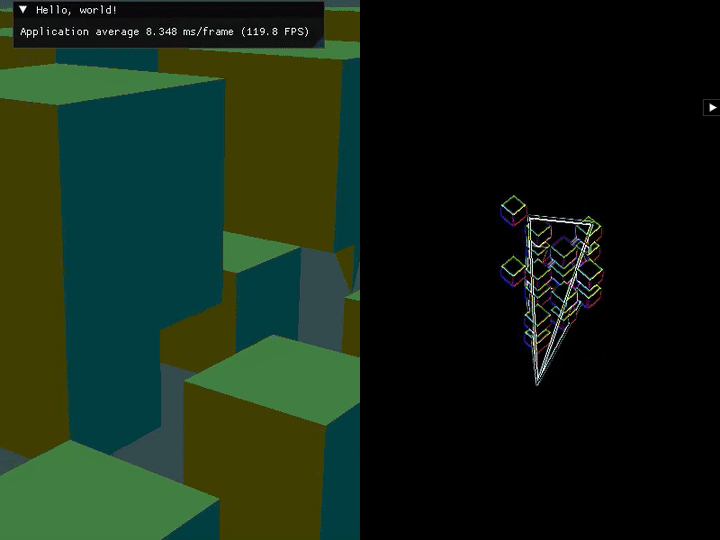
\includegraphics[width=0.45\textwidth]{frustum_cull.png}
        \caption{A visualization of frustum culling} \label{fig:cull}
\end{figure}

\begin{figure}
        \centering
        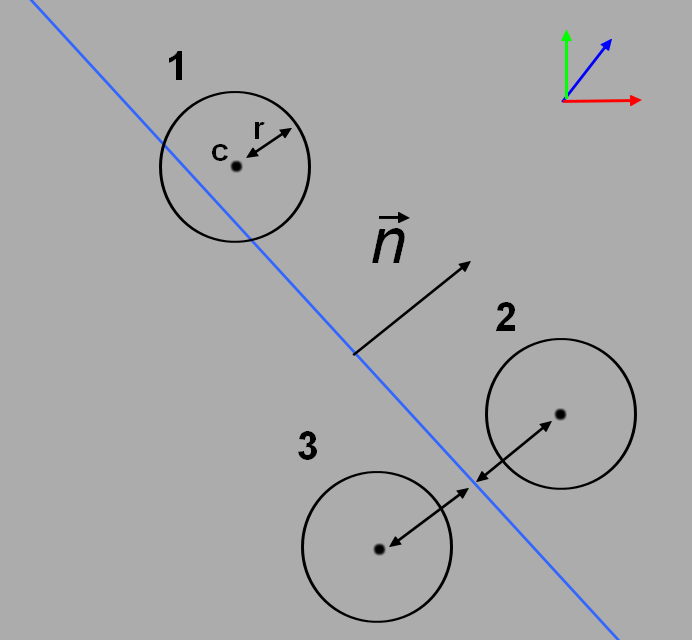
\includegraphics[width=0.35\textwidth]{sphere_detect.png}
        \caption{A sphere may be inside the plane, forward, or backward. Compare the signed distance from the sphere's center to the plane check collision with the frustum. } \label{fig:sphere}
\end{figure}


\subsubsection {CPU Frustum Culling}
CPU frustum culling implies that the draw calls are filtered by the CPU before they are issued to the GPU. Because this was implemented before instancing and indirect draw calls were added, the implementation process was easy. First, bounding volumes (collision geometry) were specified for each object in the scene. In the \texttt{Model} class, a bounding sphere with a radius equal to the distance of the model's furthest point from the origin is specified. Each camera is associated with a frustum defined by 6 planes (a normal and a distance). The \texttt{Renderer} would use the collision geometry to check if the bounding sphere of the object is partially inside the view frustum of the camera (check the signed distance of the sphere's center to the plane is greater than the negative radius of the sphere for every plane, i.e. see Fig. \ref{fig:sphere}). If it is, the draw call is issued, otherwise don't do anything. This process was repeated for every object in the scene every frame. An issue I have with this process is that the check was sequential (iterating through every object in the scene). I wanted to see if it is possible to parallelize this process and also incorporate it with instancing and indirect drawing. 

\subsubsection {GPU Frustum Culling}
I had two versions of GPU frustum culling, one unoptimized and another that was. Both incorporated instancing and indirect draws in their implementions. To start, the naive approach required a buffer containing a boolean for every instance in the scene to store the visibility of that object. A compute shader would execute the collision check for all objects (in parallel) and set their corresponding visibility bit. In the vertex shader, the index of the instance (\texttt{gl\_InstanceID}) would be used to index the visibility buffer to check if the vertex is visible. If it is, the transform of the instance is obtained and rendering goes on as usual, but if not, the vertex would be discarded. While the scene visually shows frustum culling is implemented, this process does nothing to help the performance of the renderer because the draw calls of the invisible instances are still issued to the GPU and executed. 

The issue in the first version is that the we are using instancing for the number of instances in the scene instead of the number of the instances visible in the view frustum. The second version of GPU frustum culling takes care of that by atomically accruing the count of visible instances in the culling compute shader. Instead of a buffer of booleans, it uses a buffer of indices corresponding to those of visible instances. After the buffer is computed, another shader sets the instance counts for every draw command struct in the draw command buffers of the associated model. Finally, the indirect draw call is issued to the GPU, and like before, the vertex shader will use the \texttt{gl\_InstanceID} to index the visibility buffer to obtain the transformation matrices of the instance, only this time, only the visible instances have their draw calls issued.


\subsection{Texture loading}
% Textures in the \texttt{.gltf} file format are applied per primitive of a mesh. Because of the way instancing and indirect draw batch all the mesh draw calls together and the fact that OpenGL doesn't permit the user to create an array of textures (that would be way easier to implement because the fragments would select which texture they are using), the next best way to reimplement textures was to use a texture atlas. This required the model loader to calculate the size of all textures and pack them into a single texture. Additionally, some additional computation is required to recalculate the texture coordinates of each vertex on the model. I opted to do this calculation on the GPU because it was more intuitive for me (better interface to program with). But one may also recompute the same texture coords on the CPU so that this calculation is only done once. 

\subsection {Multiple Cameras and Render Targets}
Before continuing, I should explain the architecture of the \texttt{Renderer} class itself. To begin, the \texttt{Renderer} class contains all the vertex array objects (objects that the OpenGL context use to determine the layout of the vertex stream) for each object type, the compute shaders for rendering operations (e.g. cull shaders), the uniform buffers available to every shader (e.g. camera view projection matrices) and the framebuffer textures the renderer must render onto. The renderer contains the logic to bind the appropriate data of each type of object to the OpenGL context and issue that call. The renderer also contains logic for any post-processing effects that should be applied onto the renderered image. As mentioned before, in the application mainloop, the app will blit the framebuffer textures onto the main framebuffer texture (adjacent to each other horizontally) after the render call is completed for every \texttt{Renderer} object. I am aware it may be better to have the \texttt{Renderer} specify where on the main framebuffer to write to, but I have not implemented that yet. 

This design makes it easy for me to add multiple camera views to the scene. Each camera's data lives a static vector in the \texttt{Scene} object, so if we have two \texttt{Renderer} objects, each indexing a different camera in the scene, we can render the same scene with two different perspectives and display them side by side. In addition, each renderer can add their own post-processing effects to their framebuffer textures, so the user can see the scene in different ways. It is also possible to apply these framebuffer textures onto objects in the scene (i.e. a real-time security camera monitor).

\subsection {Post-Processing}
Post-processing is when you take a rendered image (the process) and apply effects(shaders) to it (the post-process) before displaying it on the screen. As mentioned in the previous section, this is made possible through framebuffer textures in each \texttt{Renderer} object. Specifically, \texttt{Renderer} has a source texture and a destination texture. When \texttt{.render()} is called, it writes to the source texture when going through the scene. As the final step, the source texture is rendered onto a quad, the post-processing shaders are binded, and the output is written to the destination texture, which will be blitted onto the main framebuffer. To showcase the feature, I implemented a very simple edge-detection shader using kernel operators that highlights the edges of the primitives in the image. 

\subsection {Particle System and Cloth Simulation}
For the final feature to date, and for the final project of a mechanical engineering class, I implemented a cloth simulation using the Discrete Elastic Plates / Shells algorithm\cite{baraff1998large} \cite{Grinspun2003discrete}. This system was implemented on top of a base particle system interface. To me, on the basic level, a particle system is an object that manages a collection of particles (objects with a mass, position, and velocity), usually through the application of forces. At every frame of the renderer, the forces are calculated and the positions are updated and rendered. The forces also adhere to hard set of rules that help create a cohesive system.

This broad definition allows me to lump in many seemingly different effects together. For instance, streaks, stars, and smoke particle effects are no different than boids\cite{reynolds1987flocks}, fluid\cite{stam1999stable}, and cloth simulations. All these systems are governed by a set of rules that dictate the behavior and interaction of the particles. The difference is what set of rules each abide by. 

\begin{figure}
        \centering
        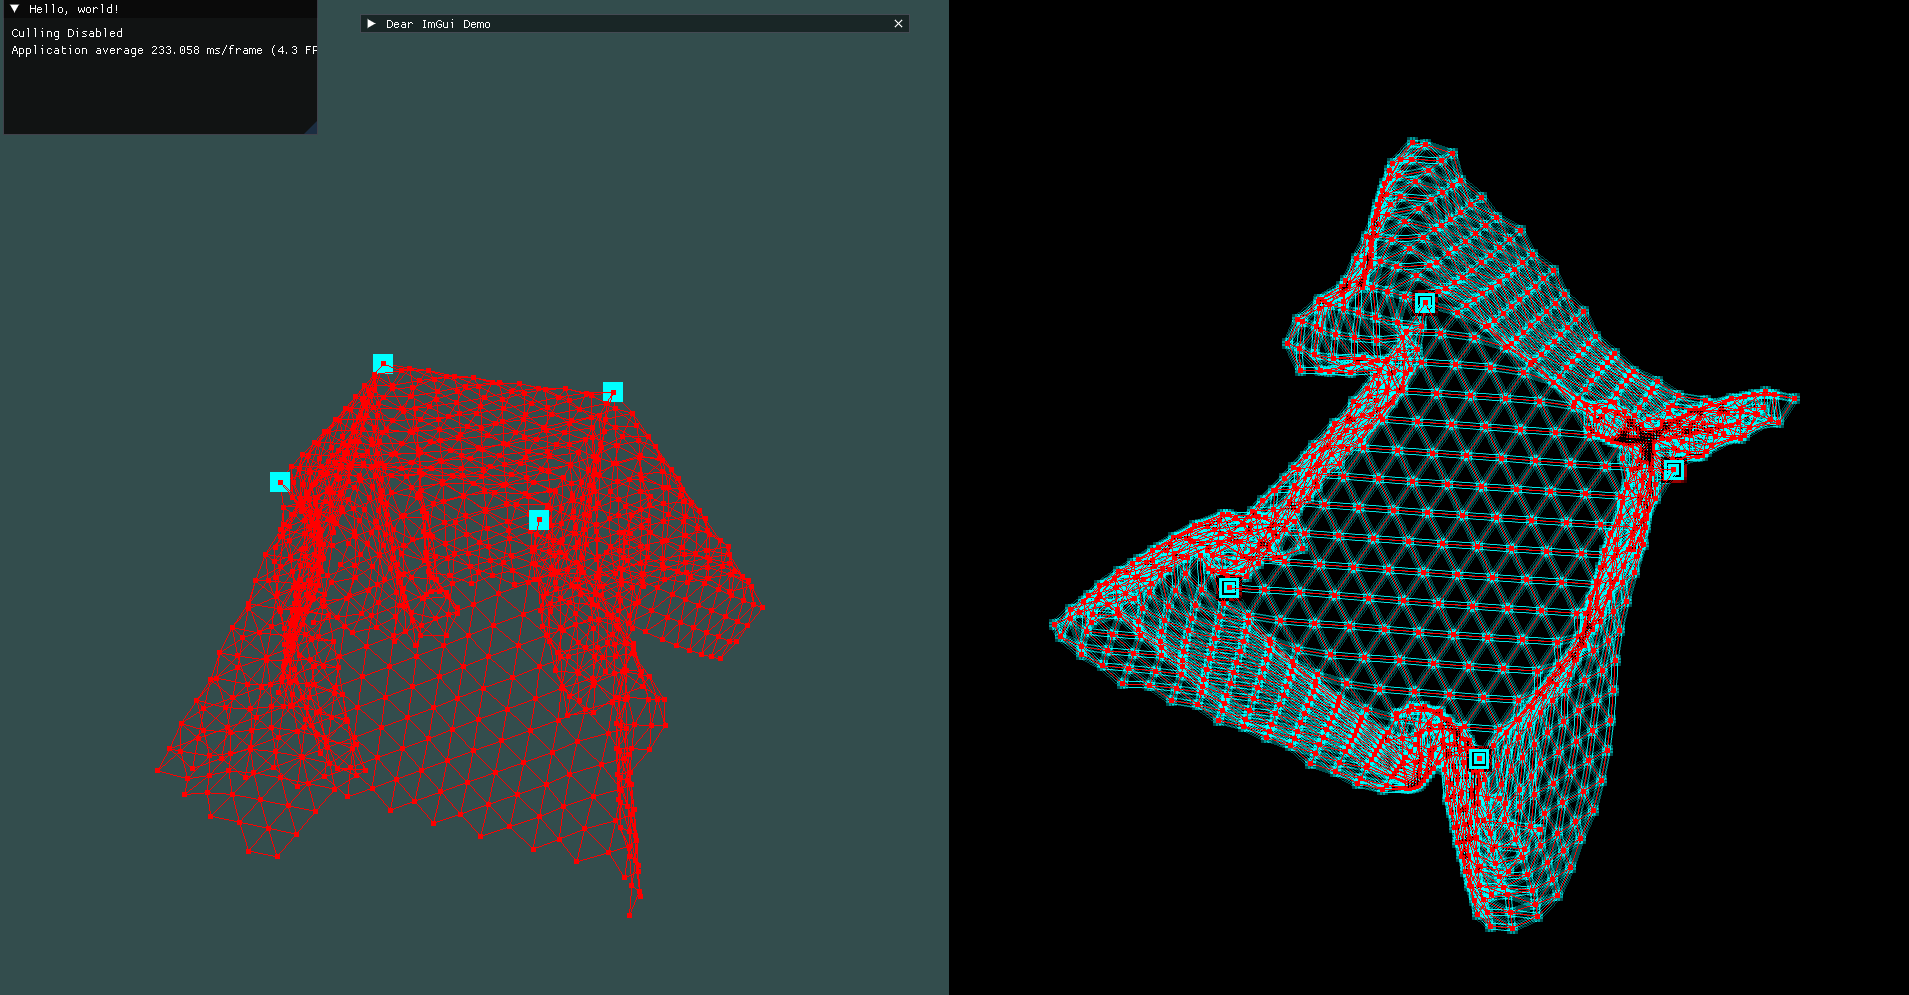
\includegraphics[width=0.45\textwidth]{cool1.PNG}
        \caption{A cloth afixed as if it were a tablecloth.} \label{fig:cloth}
\end{figure}


For the cloth simulation (see Fig. \ref{fig:cloth}), the rules are derived from the DEP/S algorithm. The algorithm is a numerical simulation algorithm that simulates the behavior of a cloth as a series of connected plates and shells (see Algorithm 1). In short, The cloth is discretized into a mesh of particles, each connected to its neighbors by edges. Elastic energy is concetrated throughout the mesh as stretching energy (from two particles pulling on each other through an edge) and bending energy (through a set of 4 particles forming a hinge to rotate about). External forces act on every particle at every frame, which provide the potential energy for the cloth to move. AlienGLRenderer implements a version of the DEP/S algorithm that uses implicit integration (Newton-Raphson method) to solve for the next position of the particles, for accuracy purposes. However, it is possible to instead use an explicit integration method (like Euler's method) for speed purposes. Additionally, it leverages the Eigen library \cite{eigen_library} to do matrix operations (OpenGL and glm does not provide functions for matrices greater than size 4) and the PARDISO library to solve the matrix system \cite{Pasadakis2023} \cite{EFTEKHARI2021101389} \cite{gaedkemerzhäuser2022}. In terms of rendering, the cloth is treated as a mesh of particles rendered as a lines connecting points. The fixed points in the simulation are highlighted with a different color to show the user where the cloth is anchored.



\section {Issues}
In the course of development of this project, I encountered a few issues that I would like to discuss. These issues that may have hindered my progress and/or still exist in the project. Regardless, I am aware of their existence and am currently figuring out whether I should solve them or not / how to solve them.

\subsection{Subtleties in OpenGL}
I was caught up in a few subtleties in OpenGL. To start, OpenGL memory alignment rules that make working with vec3s harder than it should. In the cloth simulation, the DEP algorithm assumes that the DOF vector is a $ 3 \times n $ by $ 1 $ column vector, where $n$ is the number of vertices. My initial naive implementation consisted of an array of 3 by n floats to represent the DOF vector used for calculating the forces and use the same DOF vector for drawing (specifying the vertex format to assume a vertex stream of vec3). This would work if I didn't use my DOF vector in the other (compute/debug) shaders (specifying the DOF vector as a shader buffer storage object (SSBO)).

However, according to the OpenGL specification, when using SSBOs and the std430 layout, a vec3 is aligned to 16 bytes (4 floats) in GPU memory. This means that in the shader, when I try to index into an array of vec3s, the GPU will retrieve the result with 3 floats plus 1 byte of padding. So when I copy the chunk of buffer data (the DOF vector) from CPU memory into GPU memory, I had to ensure that the total memory size of the DOF buffer is a multiple of 16 bytes. Otherwise, the GPU would read 3 floats from the buffer, skip one float part of another point, and then read the next 3 floats. This means that after my force calculation, I had to create a way to send the data to the GPU such that my buffer acted as a vector of vec4s. In other parts of the application other than the cloth simulation, you may also see me pack a struct consisting of a vec3 and a constant into a single vec4 for this reason (\texttt BoundingVolume structs in Plane and Sphere).

There is another solution to this issue without aligning the DOF vector to 16 bytes. Instead of having the GPU read the buffer as an array of vec4s/vec3s, I could pass the buffer to the GPU as an array of floats (avoiding the alignment issue entirely). Then the vertex stream for rendering for the shaders (specifically the highlight shader since the DOF positions must be read as a SSBO instead of a vertex stream) would be the indices of the particles themselves. In the highlight shader, I could use the particle indices to compute the indices of the components of each DOF for that particle. 

Another subtlety is numerous amount of calls that look-alike, but do very different things. The DOF vector in the cloth simulation is an array of double precision floats (for accuracy and precision). In the beginning, I thought, for rendering, the vertex attribute format was specified with \texttt{glVertexAttribFormat} using the type parameter \texttt{GL\_DOUBLE}. However, the correct call used to pass an array of doubles in as a vertex stream is \texttt{glVertexAttrib\textbf{L}Format} \cite{opengl_documentation}. Of course, the type cast would still need to be done in the vertex shader since the vertex shader output for positions (\texttt{gl\_Position}) is specified as a float type. I unfortunately realized this too late (it's a one character difference!), and therefore it is not implemented. 

Finally, I initially proposed to use OpenGL compute shaders to do the cloth simulation on the GPU. The DEP algorithm (save for the matrix solve) is embarassingly parallelizable, so it would be a good candidate for a compute shader. However, OpenGL does not support matrix operations beyond 4 by 4 dimensions, which means I would need to implement this myself. The conjugate gradient solve \cite{bolz2003sparse} is also a parallelizable operation, but this requires significant time to debug (and GPU debugging is much different than CPU debugging since there is no way to step through programs). I concluded that this is a huge undertaking, so I decided to stick with the CPU implementation.

\subsection{Monotlithic rendering architecture}
As more types of objects are supported by my renderer, I found the architecture of the renderer to be monolithic. This is natural since the renderer contains all the logic for rendering every single object. However, this makes adding new features to the renderer difficult. For instance, when adding support for rendering particle systems, the renderer must be have a new vertex array object for it and new logic for the rendering. I had to scroll through lots of code and make sure that my particle system rendering did not intefere with the rendering of other objects. A more pronounced example is the support for instancing and indirect draw calls with culling. Because of the way each call is structured and the way data is supplied, I had to disable materials and non instanced rendering when debugging the application. This does make sense though because these features are involved in the method of rendering objects and are core to the rendering algorithm. But if anything, a lesson learned here is echoed by a central idea: there are no zero cost abstractions \cite{caruth2019}. Because I decided to make my renderer data-oriented, I now burden myself with the explicit handling of data and all the rendering logic in the renderer. 

\subsection{Lack of oversight}
If one were to read the code for the rendering, they may get confused about why I made a few questionable decisions. For starters, I stopped implementing destructors at one point. This is because I assumed that the lifetime of my objects were the same as the lifetime of the application. This is a bad assumption to make because it is possible that the application may need to be extended to support more features, and the objects may need to be destroyed and recreated. This is especially true for the cloth simulation because it makes it impossible for me to reset the simulation without restarting the application. Because I didn't implement destructors for the cloth simulation objects, if I did delete the cloth simulation objects, there would be memory leaks (from the opengl objects not being deleted). After realizing this, I swear would never do this in production code, nor again. 

Another issue is the inconsistent usage of OpenGL types. This isn't a problem as long as my assumptions about what sizes the types I'm using align with the ground truth, or in other words, I support only a single platform. But it is important to note that C++ (as well as OpenGL) are specifications that are implemented on the platform they are running on. A \texttt{GLuint} is guaranteed to be 32 bits across all systems, but an \texttt{unsigned int} may sometimes be 64 bits or 32 bits depending on your platform's C++ implementation. This isn't a huge issue, since the intended main user of my renderer is only myself, but it is important to think about when writing production code.

\subsection{Degeneracies in the Cloth simulation}
It is known that the DEP/S algorithm is prone to some degeneracies, such as when an edge collapses or when the altitude collapses \cite{Tamstorf2013discrete}. This may manifest int the calculation as a division by zero error during the solve, an infinite loop (the error never reaches the desired tolerance), or the cloth visually becomes a cloud of points (see Fig. \ref{fig:chaos}). These may arise when the solver is unable to reach a valid solution. This is more common in simulations with more DOFs as there is more freedom for numerical instability to occur. In my own tests, the most nodes I found that would reach the resting state without reaching numerical instability is 529 nodes (1575 DOFs, side length = 22). Of course, numerical instability could be mitigated by using a smaller timestep, but this would slow down the simulation (more time steps per second and more work to compute the next position at the next second). Another potential solution would be to check the solver solution before it updates the DOF vector. If the solution is degenerate, special care can be taken (i.e. halve the time step used for the rest of the iterations). Regardless, this problem requires more investigation to find a more robust solution.



\begin{figure}
        \centering
        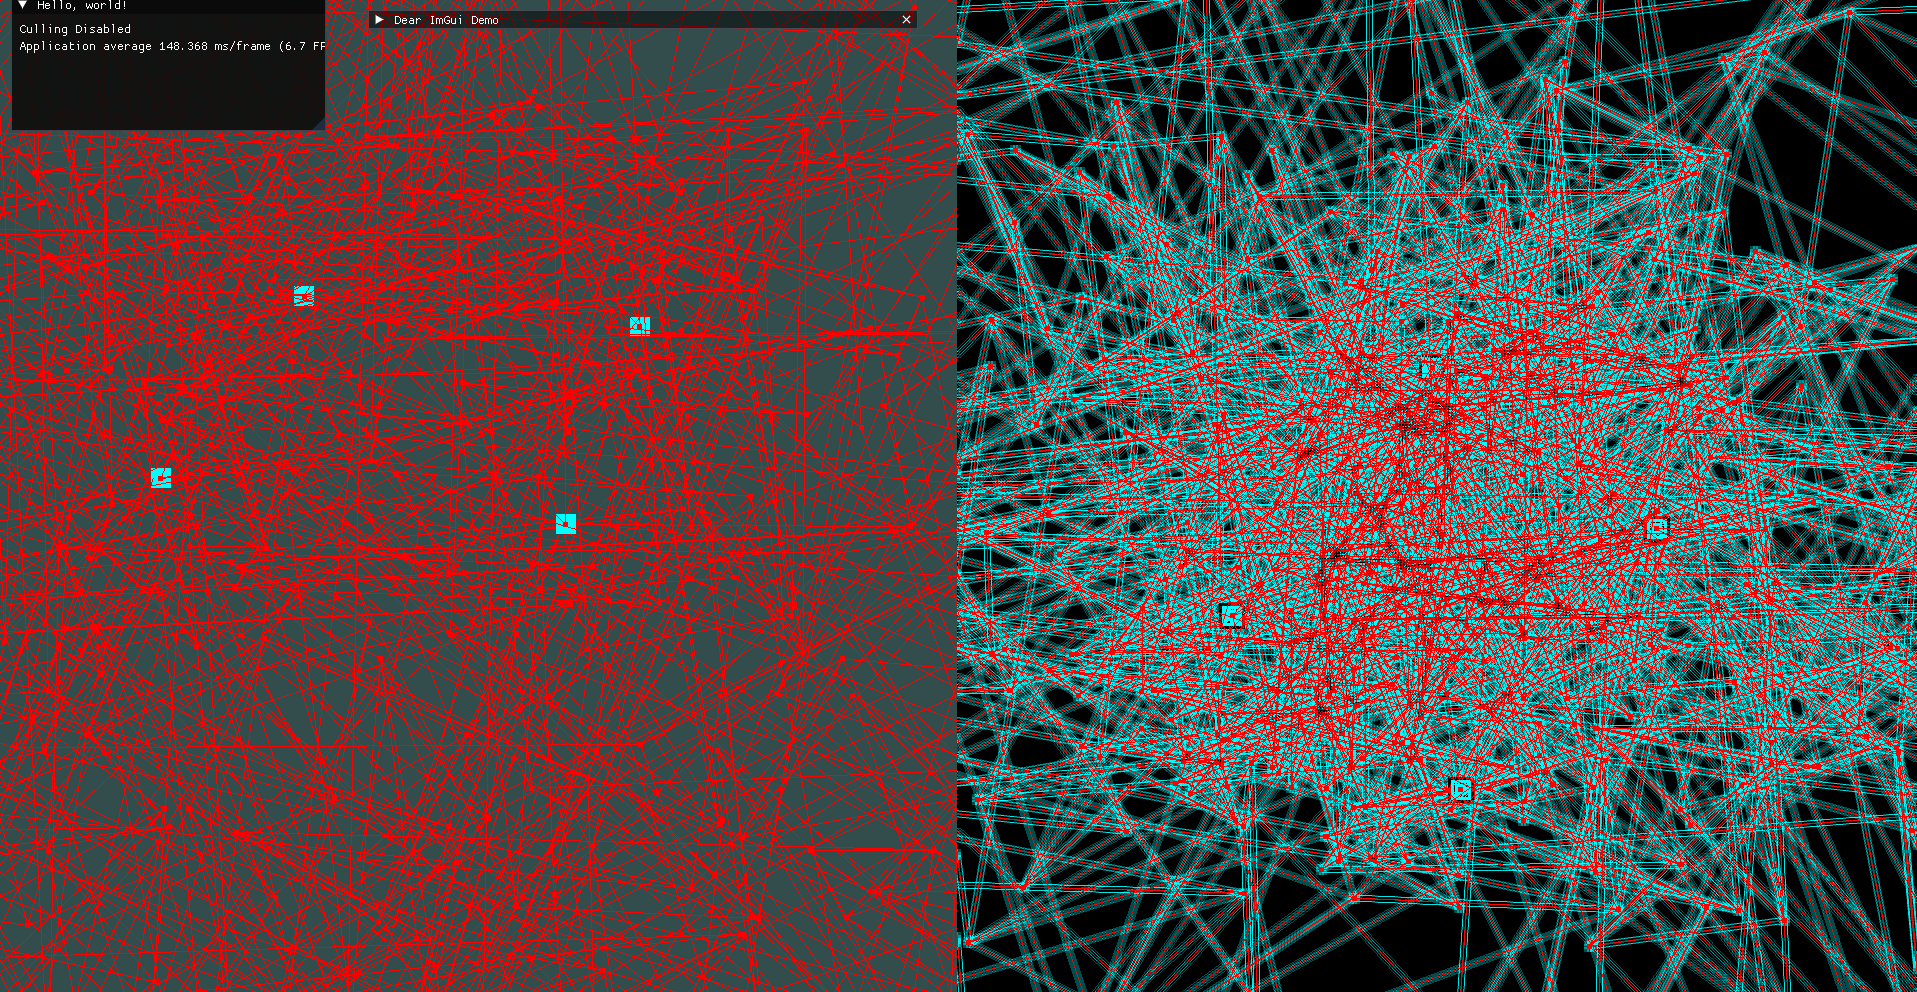
\includegraphics[width=0.5\textwidth]{chaos1.png}
        \caption{A simulation of a cloth with 576 nodes that has reached a degenerate state} \label{fig:chaos}
\end{figure}


\section {Future Work}
In addition to resolving the issues above at some point in my life, I have a few more ideas I believe the renderer would benefit from. These ideas are the following:
\begin{itemize}
        \item Implement a more robust particle system
        \item Implement occlusion culling, LOD systems, and other culling algorithms
        \item Use a triangle instead of a quad for post-processing (slightly more efficient)
        \item Implement shader graphs for post-processing
        \item Implement lighting, shadows, and reflections
        \item Implement physically based rendering and deferred shading
        \item Screen space reflections, ambient occlusion, and global illumination
        \item Rename the variables to be more descriptive
        \item Use a compute shader for the cloth simulation
        \item Implement raytracing for the renderer
        \item Use Vulkan
\end{itemize}

Each of these bullet points are a feat on their own (I am aware having all these features is overly ambitious), but I think of most interest would be the last bullet point. Vulkan \cite{Vulkan2024}, a graphics API developed and managed by the Khronos Group, is a verbose API that exposes much of the GPU's capabilities to the programmer. It is a low-level API that provides more control over the GPU pipeline, which opens up opportunities for reducing CPU overhead and optimizations. Vulkan is also a more modern API than OpenGL, and it is more likely to be supported by future hardware. But most importantly, it (along with DirectX 12, Metal, and WebGPU) are APIs that have been taking off in the industry as OpenGL is being deprecated from platforms like Apple \cite{Horwitz_2018}. I believe exposing myself to a more verbose API would further my understanding of graphics hardware more than OpenGL ever could and make me a more competitive candidate for a graphics programming position. Thus, I believe for now, the next step in my renderer may be to future proof my renderer by porting it to Vulkan.

\section {Conclusion}
In this report, I have discussed the design, implementation, and features of my capstone project, AlienGLRenderer. I have highlighted the issues I encountered during its development and what future work lies ahead, including expressing my desire to port this renderer to Vulkan. The project has been a valuable learning experience, allowing me to deepen my understanding of computer graphics and OpenGL. Moving forward, I aim to address the identified issues, implement additional features, and explore more advanced graphics APIs to further enhance the capabilities of AlienGLRenderer and my knowledge.

\section*{APPENDIX}

\onecolumn
        \begin{algorithm}[h]
                \caption{Discrete Elastic Plates}
                \textbf{Require:} $q(t_{i}), \dot{q}(t_{i})$ \hfill \texttt{DOFs and velocities at } $t_i$\\
                \hspace*{10mm} $e(m), h(n)$ \hfill \texttt{m edges and n hinges present in the plate}\\
                \hspace*{10mm} $m, M$ \hfill \texttt{masses of each particle (as a vector and matrix)}\\ 
                \hspace*{10mm} $l_{k}, k_{s}$ \hfill \texttt{undeformed length / stretching  for each edge}\\
                \hspace*{10mm} $\bar{\theta}, k_b$ \hfill \texttt{rest angles of each hinge, bending stiffness} \\                
                \hspace*{10mm} $\Delta t$ \hfill \texttt{time step}\\
                \hspace*{10mm} $\mathbf{f^{ext}}$ \hfill \texttt{external forces}\\ 
                \hspace*{10mm} \texttt{free\_index} \hfill \texttt{Index of the free DOFs}\\ \\
                \textbf{Ensure:} $q(t_{i+1}), \dot{q}(t_{i+1})$ \hfill \texttt{DOFs and velocities at } $t = t_{i+1}$\\

                \begin{algorithmic}[1]
                        \Function{Compute\_Stretching}{$q, e, l_{k}, k_{s}$}
                                \State $\mathbf{f^{stretch}},\mathbf{J^{stretch}}  \gets 0, 0$ \hfill \texttt{Initialize}
                                \For{$i \gets 1$ to $m$}
                                        \State \texttt{x0}, \texttt{x1} $\gets q(e(k, 1)), \, q(e(k, 2))$ \hfill \texttt{Get DOFs of particles in edges}
                                        \State $\mathbf{f^{grad}}, \mathbf{J^{hess}} \gets \Call{GradEs\_HessEs}{\texttt{x0}, \texttt{x1}, l_{k}(i), k_{s}(i)}$ \hfill Refer to Appendix of \cite{jawedlimdiscrete} \\
                                        \State $\mathbf{f^{stretch}}(e(k)) \gets \mathbf{f^{stretch}}(e(k)) - \mathbf{f^{grad}}$ \hfill \texttt{Update total force/Jacobian}
                                        \State $\mathbf{J^{stretch}}(e(k), e(k)) \gets \mathbf{J^{stretch}}(e(k), e(k)) - \mathbf{J^{hess}}$
                                \EndFor
                                \State \Return $\mathbf{f^{stretch}}, \mathbf{J^{stretch}}$
                        \EndFunction \\ 
                
                        \Function{Compute\_Bending}{$q, h, k_b$}
                                \State $\mathbf{f^{bend}},\mathbf{J^{bend}}  \gets 0, 0$ \hfill \texttt{Initialize}
                                \For{$i \gets 1$ to $n$}
                                        \State \texttt{x0}, \texttt{x1}, \texttt{x2}, \texttt{x3} $\gets q(e(k, 1)), \,  q(e(k, 2)), \, q(e(k, 3)), \, q(e(k, 4))$ \hfill \texttt{Get DOFs of particles in hinges}
                                        \State $\mathbf{f^{grad}}, \mathbf{J^{hess}} \gets \Call{GradEb\_HessEb}{\texttt{x0}, \texttt{x1}, \texttt{x2}, \texttt{x3}, l_{k}(i), k_{s}(i)}$ \hfill Refer to Appendix of \cite{jawedlimdiscrete} \\
                                        \State $\mathbf{f^{bend}}(e(k)) \gets \mathbf{f^{bend}}(e(k)) - \mathbf{f^{grad}}$ \hfill \texttt{Update total force/Jacobian}
                                        \State $\mathbf{J^{bend}}(e(k), e(k)) \gets \mathbf{J^{bend}}(e(k), e(k)) - \mathbf{J^{hess}}$
                                \EndFor
                                \State \Return $\mathbf{f^{bend}}, \mathbf{J^{bend}}$
                        \EndFunction \\
                
                \Function{Discrete\_Elastic\_Plates}{$q, \dot{q}$} 
                    \State Guess: $q^{(1)}(t_{i+1}) \gets q(t_i)$
                    \State $n \gets 1$
                    \While{$\text{error} > \text{tolerance}$} \\
                        \State $\mathbf{f^{stretch}}, \mathbf{J^{stretch}}  \gets \Call{Compute\_Stretching}{q, e, l_{k}, k_{s}}$ 

                        \State $\mathbf{f^{bend}}, \mathbf{J^{bend}}  \gets \Call{Compute\_Bending}{q, e, l_{k}, k_{s}}$ \\
                                
                        \State $\mathbf{f^{tot}} \gets \mathbf{f^{bend}} + \mathbf{f^{stretch}} + \mathbf{f^{ext}}$ \hfill \texttt{Aggregate forces}
                        \State $\mathbf{f} \gets \frac{1}{\Delta t}m \odot \left[\frac{1}{\Delta t} \left[q^{(n)} - q^{(1)}\right] - \dot{q} \right] - \mathbf{f^{tot}}$ \\

                        \State $\mathbf{J^{tot}} \gets \mathbf{J^{bend}} + \mathbf{J^{stretch}}$ \hfill \texttt{Aggregate Jacobians}
                        \State $\mathbf{J} \gets \frac{1}{\Delta t} M - \mathbf{J^{tot}}$ \\
                        
                        \State $\mathbf{f}_\text{free} \gets \mathbf{f}(\texttt{free\_index})$
                        \State $\mathbf{J}_\text{free} \gets \mathbf{J}(\texttt{free\_index}, \texttt{free\_index})$\\
                        \State $\Delta q_\text{free} \gets \mathbf{J}_\text{free}^{-1} \mathbf{f}_\text{free}$
                        \State $q^{(n+1)}(\texttt{free\_index}) \gets q^{(n)}(\texttt{free\_index}) - \Delta q_\text{free}$ \hfill \texttt{Update free DOFs}
                        \State $\text{error} \gets \text{sum}(\lvert \mathbf{f}_\text{free} \rvert)$
                        \State $n \gets n + 1$ \\
                    \EndWhile
                    \State $q(t_{i+1}) \gets q^{(n)}(t_{i+1})$                  \hfill \texttt{Update DOFs for next time step}
                    \State $\dot{q}(t_{i+1}) \gets \dot{q}^{(n)}(t_{i+1})$
                \EndFunction
                \end{algorithmic}
                \end{algorithm}
        % \end{figure*}
\twocolumn




\addtolength{\textheight}{-12cm}   % This command serves to balance the column lengths
                                  % on the last page of the document manually. It shortens
                                  % the textheight of the last page by a suitable amount.
                                  % This command does not take effect until the next page
                                  % so it should come on the page before the last. Make
                                  % sure that you do not shorten the textheight too much.

%%%%%%%%%%%%%%%%%%%%%%%%%%%%%%%%%%%%%%%%%%%%%%%%%%%%%%%%%%%%%%%%%%%%%%%%%%%%%%%%



%%%%%%%%%%%%%%%%%%%%%%%%%%%%%%%%%%%%%%%%%%%%%%%%%%%%%%%%%%%%%%%%%%%%%%%%%%%%%%%%

\bibliographystyle{ieeetr} % We choose the "plain" reference style
\bibliography{refs} % Entries are in the refs.bib file

\end{document}
